% Chapter 2
\chapter{Writing Installation XML Files}

% What you need
\section{What You Need}

\subsection{Your editor}

In order to write your XML installation files, you just need a plain
text editor. Of course it's always easier to work with color coded text,
so you might rather want to work with a text editor having such a
feature. Here is a list of free editors that work well :
\begin{itemize}
  \item Jext : \url{http://www.jext.org/}
  \item JEdit : \url{http://www.jedit.org/}
  \item classics like Vim and (X)Emacs.
\end{itemize}\

\subsection{Writing XML}

Though you might not know much about XML, you have certainly heard about
it. If you know XML you can skip this subsection as we will briefly
present how to use XML.\\

XML is a markup language, really close to HTML. If you've ever worked
with HTML the transition will be fast. However there are a few little
things to know. The markups used in XML have the following form :
\texttt{<markup>}. Each markup has to be closed somewhere with its
ending tag : \texttt{</markup>}. Each tag can contain text and other
markups. If a markup does not contain anything, it is just reported once
: \texttt{<markup/>}. A markup can contain attributes like :
\texttt{<markup attr1="123" attr2="hello !"/>}. Here is a sample of a
valid XML structure :
\footnotesize
\begin{verbatim}
<chapter title="Chapter 1">
  <section name="Introduction">
    <paragraph>
    This is the text of the paragraph number 1. It is available for the very low
    price of <price currency="dollar">1 000 000</price>.
    </paragraph>
  </section>
  <section name="xxx">
  xxx
  </section>
</chapter>
\end{verbatim}
\normalsize

You should be aware of the following common mistakes :
\begin{itemize}

  \item markups \textbf{are} case sensitive : \texttt{<markup>} is different
  from \texttt{<Markup>}.

  \item you \textbf{must} close the markups in the same order as you create them
  : \texttt{<m1><m2>(...)</m2></m1>} is right but
  \texttt{<m1><m2>(...)</m1></m2>} is not.

\end{itemize}

Also, an XML file must start with the following header :\\
\texttt{<?xml version="1.0" encoding="iso-8859-1 standalone="yes" ?>}. The only
thing you should modify is the encoding (put here the one your text editor saves
your files to). The \texttt{standalone} attribute is not very important for
us.\\

This (brief !) introduction to XML was just meant to enable you to write
your installation specification. For a better introduction there are
plenty of books and articles/tutorials dealing with XML on the Internet,
in book stores, in magazines and so on.\\

% Built-in variables
\section{Variable Substitution}

During the installation process IzPack can substitute variables in
various places with real values. Obvious targets for variable
substitution are resource files and launch scripts, however you will
notice many more places where it is more powerful to use variables
rather then hard coded values. Wherever variables can be used it will
be explained in the documentation.\\

There are three types of variables:
\begin{itemize}
  \item Built-In variables. These are implemented in IzPack and are
        all dynamic in nature. This means that the value of each
        variable depends on local conditions on the target system.
  \item Environment variables. These are provided by the operating system the
        installer is run on.
  \item Variables that you can define. You also define the value,
        which is fixed for a given installation file.
\end{itemize}

You define your own variables in the installation XML file with the
\texttt{<variable>} tag. How to do this is explained in detail later in
this chapter.\\

\textbf{Please note} that when using variables they must always appear
with a '\texttt{\$}' sign as the first character, even though they are
not defined this way.\\

\subsection{The Built-In Variables}
The following variables are built-in :
\begin{itemize}
  \item \texttt{\$INSTALL\_PATH} : the installation path on the
        target system, as chosen by the user
  \item \texttt{\$APPLICATIONS\_DEFAULT\_ROOT} : the default path for
        applications
  \item \texttt{\$JAVA\_HOME} : the \Java virtual machine home path
  \item \texttt{\$USER\_HOME} : the user's home directory path
  \item \texttt{\$USER\_NAME} : the user name
  \item \texttt{\$APP\_NAME} : the application name
  \item \texttt{\$APP\_URL} : the application URL
  \item \texttt{\$APP\_VER} : the application version
  \item \texttt{\$ISO3\_LANG} : the ISO3 language code of the selected langpack.
  \item \texttt{\$FILE\_SEPARATOR} : the file separator on the installation system
\end{itemize}\

\subsection{Environment Variables}
Environment variables can be accessed via the syntax \texttt{\$\{ENV[variable]\}}. 
The curly braces are mandatory.
Note that variable names are case-sensitive and usually in UPPER CASE.

Example: To get the value of the OS environment variable "CATALINA\_HOME", use \texttt{\$\{ENV[CATALINA\_HOME]\}}.

\subsection{Parse Types}
Parse types apply only when replacing variables in text files. At places
where it might be necessary to specify a parse type, the documentation
will mention this. Depending on the parse type, IzPack will handle
special cases -such as escaping control characters- correctly. The
following parse types are available:
\begin{itemize}
  \item \texttt{plain} - use this type for plain text files, where no
        special substitution rules apply. All variables will be
        replaced with their respective values as is.
  \item \texttt{javaprop} - use this type if the substitution happens
        in a Java properties file. Individual variables might be
        modified to function properly within the context of Java
        property files.
  \item \texttt{xml} - use this type if the substitution happens in
        a XML file. Individual variables might be modified to function
        properly within the context of XML files.
  \item \texttt{shell} - use this type if the substitution happens in
        a shell script. Because shell scripts use \texttt{\$variable}
        themselves, an alternative variable marker is used:
        \texttt{\%variable} or \texttt{\%\{variable\}}.
\end{itemize}

% The IzPack elements
\section{The \IzPack Elements}

\noindent
\textit{When writing your installer XML files, it's a good idea to have a look
at the \IzPack installation DTD}.\\

\subsection{The Root Element \texttt{<installation>}}
\label{root-element}

The root element of an installation is \texttt{<installation>}. It takes
one required attribute : \texttt{version}. The attribute defines the
version of the XML file layout and is used by the compiler to identify
if it is compatible with the XML file. This should be set to $1.0$ for
the moment.\\

\subsection{The Information Element \texttt{<info>}}
\label{info-element}

This element is used to specify some general information for the installer. It
contains the following elements :
\begin{itemize}

  \item \texttt{<appname>} : the application name
  \item \texttt{<appversion>} : the application version
  \item \texttt{<appsubpath>} : the subpath for the default of the installation path.
  A variable substitution and a maskable slash-backslash conversion will be done. If this
  tag is not defined, the application name will be used instead.
  \item \texttt{<url>} : the application official website url
  \item \texttt{<authors>} : specifies the author(s) of the application. It must contain
  at least one \texttt{<author>} element whose attributes are :
  \begin{itemize}
    \item \texttt{name} : the author's name
    \item \texttt{email} : the author's email
  \end{itemize}
  \item \texttt{<uninstaller>} : specifies whether to create an uninstaller after installation, and which name to use for it. This tag has the \texttt{write} attribute, with default value \texttt{yes}. If this tag is not specified, the uninstaller will still be written. The \texttt{name} attribute can be used to change the default name of the generated uninstaller, \textit{i.e.} \texttt{uninstaller.jar}.
  \item \texttt{<javaversion>} : specifies the minimum version of Java required to install your program. Values can be \texttt{1.2}, \texttt{1.2.2}, \texttt{1.4}, etc. The test is a lexical comparison against the \texttt{java.version} System property on the install machine.
  \item \texttt{<webdir>} : Causes a ``web installer'' to be created, and specifies the URL packages are retrieved from at install time. The content of the tag must be a properly formed URL. See section~\ref{webinstaller} for more details.

\end{itemize}\

Here is an example of a typical \texttt{<info>} section :\\
\footnotesize
\begin{verbatim}
<info>
  <appname>Super extractor</appname>
  <appversion>2.1 beta 6</appversion>
  <appsubpath>myCompany/SExtractor</appsubpath>
  <url>http://www.superextractor.com/</url>
  <authors>
    <author name="John John Doo" email="jjd@jjd-mail.com"/>
    <author name="El Goyo" email="goyoman@mymail.org"/>
  </authors>
  <javaversion>1.2</javaversion>
</info>
\end{verbatim}
\normalsize

\subsection{The Variables Element \texttt{<variables>}}
\label{variables-element}

This element allows you to define variables for the variables
substitution system. Some variables are built-in, such as
\texttt{\$INSTALL\_PATH} (which is the installation path chosen by the
user). When you define a set of variables, you just have to place as
many \texttt{<variable>} tags in the file as needed. If you define a
variable named \texttt{VERSION} you need to type \$VERSION in the files
to parse. The variable substitutor will then replace it with the correct
value. One \texttt{<variable>} tag take the following attributes :
\begin{itemize}

  \item \texttt{name} : the variable name
  \item \texttt{value} : the variable value

\end{itemize}\

Here's a sample \texttt{<variables>} section :\\
\footnotesize
\begin{verbatim}
<variables>
  <variable name="app-version" value="1.4"/>
  <variable name="released-on" value="08/03/2002"/>
</variables>
\end{verbatim}
\normalsize

\subsection{The GUI Preferences Element \texttt{<guiprefs>}}
\label{guiprefs-element}

This element allows you to set the behavior of your installer GUI. This
information will not have any effect on the command-line installers that will be
available in future versions of \IzPack. The arguments to specify are :
\begin{itemize}

  \item \texttt{resizable} : takes \texttt{yes} or \texttt{no} and indicates
  whether the window size can be changed or not.
  \item \texttt{width} : sets the initial window width
  \item \texttt{height} : sets the initial window height.

\end{itemize}\

Here's a sample :
\footnotesize
\begin{verbatim}
<guiprefs resizable="no" width="800" height="600"/>
\end{verbatim}
\normalsize

Starting from IzPack 3.6, the look and feel can be specified in this section on
a per-OS basis. For instance you can use the native look and feels on Win32 and
OS X but use a third-party one on Unix-like platforms. To do that, you have to
add some children to the \texttt{guiprefs} tag:
\begin{itemize}

  \item \texttt{laf}: the tag that specifies a look and feel. It has a
  \texttt{name} parameter that defines the look and feel name.
  \item Each \texttt{laf} element needs at least one \texttt{os} tag, specified
  like in the other parts of the specification that support this tag.
  \item Like you can add \texttt{os} elements, you can add any number of
  \texttt{param} elements to customize a look and feel. A \texttt{param}
  elements has two attribues: \texttt{name} and \texttt{value}.

\end{itemize}\

The available look and feels are:
\begin{itemize}

  \item Kunststoff: \texttt{kunststoff}
  \item Liquid: \texttt{liquid}
  \item Metouia: \texttt{metouia}
  \item JGoodies Looks: \texttt{looks}

\end{itemize}\

If you don't specify a look and feel for a particular operating system, then the
default native one will be used: Windows on Windows, Aqua on Mac OS X and Metal
on the Unix-like variants.\\

The \textit{Liquid Look and Feel} supports the following parameters:
\begin{itemize}

  \item \texttt{decorate.frames}: \texttt{yes} means that it will render the
  frames in Liquid style
  \item \texttt{decorate.dialogs}: \texttt{yes} means that it will render the
  dialogs in Liquid style

\end{itemize}\

The \textit{JGoodies Looks} look and feel can be specified by using the
\texttt{variant} parameters. The values can be one of:
\begin{itemize}

  \item \texttt{extwin}: use the Windows Extension look
  \item \texttt{plastic}: use the basic Plastic look
  \item \texttt{plastic3D}: use the Plastic 3D look
  \item \texttt{plasticXP}: use the Plastic XP look (default).

\end{itemize}\

Here is a small sample:
\begin{verbatim}
<guiprefs height="600" resizable="yes" width="800">
    <laf name="metouia">
        <os family="unix" />
    </laf>
    <laf name="looks">
        <os family="windows" />
        <param name="variant" value="extwin" />
    </laf>
</guiprefs>
\end{verbatim}

Starting from IzPack 3.7, some characteristics can be customized with the
\texttt{<modifier>} tag which contains following attributes:
\begin{itemize}

  \item \texttt{key}: a well defined key of the characteristic which should
  be changed.
  \item \texttt{value} the value for the key.
\end{itemize}\
Following key value pairs are defined:
\begin{itemize}
\item \texttt{useButtonIcons}: possible are "yes" or "no". Default is "yes".
If it is set to "no", all buttons which are created via the ButtonFactory
contains no icon also a icon id was submitted. Directly created buttons are
not affected.
\item \texttt{useLabelIcons}: possible are "yes" or "no". Default is "yes".
If it is set to "no", all labels which are created via the LabelFactory
contains no icon also a icon id was submitted. Directly created labels are
not affected.
\item \texttt{useFlags}: possible are "yes" or "no". Default is "yes".
If it is set to "no", no flag will be displayed in the language selection
dialog. For "no" it is recomanded to define also langDisplayType other then
"iso3".
\item \texttt{langDisplayType}: possible are "iso3", "native" and "default".
Default is "iso3". With "iso3" the text for a language will be displayed as
ISO 639-2:1998 code. With "native" the notation of the language will be used
if possible, else the notation of the default locale. Using "default" will
be presented the language in the notation of the default locale of the VM.
\end{itemize}\

Here is a small sample:
\begin{verbatim}
<guiprefs width="640" height="480" resizable="no">
    <modifier key="useButtonIcons" value="no"/>
    <modifier key="useLabelIcons" value="no"/>
    <modifier key="useFlags" value="no"/>
    <modifier key="langDisplayType" value="native"/>
</guiprefs>
\end{verbatim}

\subsection{The Localization Element \texttt{<locale>}}
\label{localization-element}

This element is used to specify the language packs (langpacks) that you want to
use for your installer. You must set one \texttt{<langpack>} markup per
language. This markup takes the \texttt{iso3} parameter which specifies the iso3
language code.\\

Here's a sample :\\
\footnotesize
\begin{verbatim}
<locale>
  <langpack iso3="eng"/>
  <langpack iso3="fra"/>
  <langpack iso3="spa"/>
</locale>
\end{verbatim}\
\normalsize

The supported ISO3 codes are :
\begin{center}
\begin{tabular}{|l|l|}
\hline
\textit{ISO3 code} & \textit{Language} \\ \hline
cat & Catalunyan \\ \hline
chn & Chinese \\ \hline
cze & Czech \\ \hline
dan & Danish \\ \hline
deu & German \\ \hline
eng & English \\ \hline
fin & Finnish \\ \hline
fra & French \\ \hline
hun & Hungarian \\ \hline
ita & Italian \\ \hline
jpn & Japanese \\ \hline
mys & Malaysian \\ \hline
ned & Nederlands \\ \hline
nor & Norwegian \\ \hline
pol & Polnish \\ \hline
por & Portuguese (Brazilian) \\ \hline
rom & Romanian \\ \hline
rus & Russian \\ \hline
scg & Serbian \\ \hline
spa & Spanish \\ \hline
svk & Slovakian \\ \hline
swe & Swedish \\ \hline
ukr & Ukrainian \\ \hline
\end{tabular}\
\end{center}

\subsection{The Resources Element \texttt{<resources>}}
\label{resources-element}

Several panels, such as the license panel and the shortcut panel,
require additional data to perform their task. This data is supplied
in the form of resources. This section describes how to specify
them. Take a look at each panel description to see if it might need
any resources. Currently, no checks are made to ensure resources
needed by any panel have been included. The \texttt{<resources>}
element is not required, and no \texttt{<res>} elements are required
within.\\

You have to set one \texttt{<res>} markup for each resource. Here are
the attributes to specify :
\begin{itemize}

  \item \texttt{src} : the path to the resource file which can be named freely
  of course (for instance \texttt{my-picture.jpg}).
  \item \texttt{id} : the resource id, depending on the needs of a particular panel
  \item \texttt{parse} : takes \texttt{yes} or \texttt{no} (default is
  \texttt{no}) - used to specify whether the resource must be parsed at the
  installer compilation time. For instance you could set the application version
  in a readme file used by \texttt{InfoPanel}.
  \item \texttt{type} : specifies the parse type. This makes sense only for a text
  resource  - the default is \texttt{plain}, other values are \texttt{javaprop,
  xml} (Java properties file and XML files)
  \item \texttt{encoding} : specifies the resource encoding if the receiver needs
  to know. This makes sense only for a text resource.

\end{itemize}\

Here's a sample :
\footnotesize
\begin{verbatim}
<resources>
  <res id="InfoPanel.info" src="doc/readme.txt" parse="yes"/>
  <res id="LicencePanel.licence" src="legal/License.txt"/>
</resources>
\end{verbatim}
\normalsize

\subsection{The Panels Element \texttt{<panels>}}
\label{panels-element}

Here you tell the compiler which panels you want to use. They will
appear in the installer in the order in which they are listed in your
XML installation file. Take a look at the different panels in order to
find the ones you need. The \texttt{<panel>} markup takes a single
attribute \texttt{classname} which is the classname of the panel.\\

Here's a sample :
\footnotesize
\begin{verbatim}
<panels>
  <panel classname="HelloPanel"/>
  <panel classname="LicencePanel"/>
  <panel classname="TargetPanel"/>
  <panel classname="InstallPanel"/>
  <panel classname="FinishPanel"/>
</panels>
\end{verbatim}
\normalsize

\subsection{The Packs Element \texttt{<packs>}}
\label{packs-element}

This is a crucial section as it is used to specify the files that need
to be installed. The \texttt{<packs>} section consists of several
\texttt{<pack>} tags.

The \texttt{<pack>} takes the following attributes :
  \begin{itemize}
    \item \texttt{name}: the pack name
    \item \texttt{required}: takes \texttt{yes} or \texttt{no} and specifies
    whether the pack is optional or not.
    \item \texttt{os}: optional attribute that lets you make the pack targeted
    to a specific \textsl{operating system}, for instance \texttt{unix},
    \texttt{mac} and so on.
    \item \texttt{preselected}: optional attribute that lets you choose whether
    the pack is by default selected for installation or not. Possible values
    are \texttt{yes} and \texttt{no}. A pack which is not preselected needs to
    be explicitly selected by the user during installation to get installed.
    \item \texttt{loose}: can be used so that the files are not located in the
    installer Jar. The possible values are \texttt{true} or \texttt{false}, the
    default beeing \texttt{false}. The author of this feature needed to put his
    application on a CD so that the users could run it directly from this media.
    However, he also wanted to offer them the possibility to install the
    software localy. Enabling this feature will make IzPack take the files on
    disk instead of from the installer. \textit{Please make sure that your relative
    files paths are correct !}
    \item \texttt{id}: this attribute is used to give a unique id to the pack to
    be used for internationalization.
  \end{itemize}

\subsubsection{Internationalization of the PacksPanel}
In order to provide internationalization for the PacksPanel, so that your users can
be presented with a different name and description for each language you support,
 you have to create a file named \texttt{packsLang.xml\_xyz} where \texttt{xyz}
 is the ISO3 code of the language in lowercase. Please be aware that case is significant.
 This file has to be inserted in the resources section of \texttt{install.xml} with the
 \texttt{id} and \texttt{src} attributes set at the name of the file. The format of
 these files is identical with the distribution langpack files located at
 \texttt{\$IZPACK\_HOME/install/langpacks/installer}. For the name of the panel you just
 use the pack \texttt{id} as the txt \texttt{id}. For the description you use the pack
 \texttt{id} suffixed with \texttt{'.description'}.

The following sections describe the tags available for a \texttt{<pack>} section.

\subsubsection{\texttt{<description>} - pack description}

The contents of the \texttt{<description>} tag describe the pack contents.
This description is displayed if the user highlights the pack during
installation.

\subsubsection{\texttt{<depends>} - pack dependencies}
This can be used to make this pack selectable only to be installed only if some other is
selected to be installed. The pack can depend on more than one by specifying more than one
\texttt{<depends>} elements.\\
Circular depedencies are not supported and the compiler reports an error if one occurs.

This tag takes the following attribute:
\begin{itemize}
\item \texttt{packname}: The name of the pack that it depends on
\end{itemize}

\subsubsection{\texttt{<os>} - OS restrictions}

It is possible to restrict a panel to a certain list of operating systems. This
tag takes the following attributes:
\begin{itemize}
\item \texttt{family}: unix, windows or mac
\item \texttt{name}: the exact OS name (ie Windows, Linux, ...)
\item \texttt{version}: the exact OS version (see the JVM \texttt{os.version} property)
\item \texttt{arch}: the machine architecture (see the JVM \texttt{os.arch} property).
\end{itemize}

\subsubsection{\texttt{<updatecheck>}}

This feature can update an already installed package, therefore removing
superfluous files after installation. Here's how this feature author (Tino Schwarze)
described it on the IzPack development mailing-list:
\begin{quote}
Each pack can now
specify an \texttt{<updatecheck>} tag. It supports a subset of ant fileset
syntax, e.g.:
\begin{verbatim}
<updatecheck>
  <include name="lib/**" />
  <exclude name="config/local/** />
</updatecheck>
\end{verbatim}\

If the paths are relative, they will be matched relative to
\texttt{\$INSTALL\_PATH}. Update checks are only enabled if at least one
\texttt{<include>} is specified. See
\texttt{com.izforge.izpack.installer.Unpacker} for details.
\end{quote}

\subsubsection{\label{tag:file}\texttt{<file>} - add files or directories}

The \texttt{<file>} tag specifies a file (a directory is a file too) to
include into the pack. It takes the following attributes:

\begin{itemize}

  \item \texttt{src}: the file location (relative path) - if this is a
  directory its content will be added recursively

  \item \texttt{targetdir}: the destination directory, could be something like
  \texttt{\$INSTALL\_PATH/subdirX}

  \item \texttt{os}: can optionally specify a target operating system
  (\texttt{unix, windows, mac}) - this means that the file will only be
  installed on its target operating system

  \item \texttt{override}: if \texttt{true} then if the file is already
  installed, it will be overwritten. Alternative values: \texttt{asktrue} and
  \texttt{askfalse} -- ask the user what to do and supply default value for
  non-interactive use. Another possible values is \texttt{update}. It means
  that the new file is only installed if it's modification time is newer than
  the modification time of the already existing file (note that this is not a
  reliable mechanism for updates - you cannot detect whether a file was
  altered after installation this way.) By default it is set to \texttt{update}.

\end{itemize}
\paragraph{\label{tag:additionaldata}\texttt{<additionaldata>}}

This tag can also be specified in order to pass additional data
related to a file tag for customizing.

\begin{itemize}

  \item \texttt{<key>}: key to identify the data
  \item \texttt{<value>}: value which can be used by a custom
  action

\end{itemize}

\subsubsection{\label{tag:singlefile}\texttt{<singlefile>} - add a single file}

Specifies a single file to include. The difference to \texttt{<file>} is that
this tag allows the file to be renamed, therefore it has a
\texttt{target} attribute instead of \texttt{targetdir}.

\begin{itemize}

  \item \texttt{src}: the file location (relative path)

  \item \texttt{target}: the destination file name, could be something
  like \texttt{\$INSTALL\_PATH/subdirX/fileY}

  \item \texttt{os}: can optionally specify a target operating system
  (\texttt{unix, windows, mac}) - this means that the file will only be
  installed on its target operating system

  \item \texttt{override}: see \texttt{<file>} (\ref{tag:file}) for description

\end{itemize}
A \texttt{<additionaldata>} (\ref{tag:additionaldata}) tag can
also be specified for customizing.

\subsubsection{\label{tag:fileset}\texttt{<fileset>}: add a fileset}

The \texttt{<fileset>} tag allows files to be specified using the powerful
Jakarta Ant set syntax. It takes the following parameters:

\begin{itemize}

  \item \texttt{dir}: the base directory for the fileset (relative path)

  \item \texttt{targetdir}: the destination path, works like for
  \texttt{<file>}

  \item \texttt{casesensitive}: optionally lets you specify if the names
  are case-sensitive or not - takes \texttt{yes} or \texttt{no}

  \item \texttt{defaultexcludes}: optionally lets you specify if the default
  excludes will be used - takes \texttt{yes} or \texttt{no}.

  \item \texttt{os}: specifies the operating system, works like for
  \texttt{<file>}

  \item \texttt{override}: see \texttt{<file>} for description

  \item \texttt{includes}: comma- or space-separated list of patterns of
  files that must be included; all files are included when omitted.
  This is an alternative for multiple include tags.

  \item \texttt{excludes}: comma- or space-separated list of patterns of
  files that must be excluded; no files (except default excludes) are
  excluded when omitted. This is an alternative for multiple exclude tags.

\end{itemize}

You specify the files with  \texttt{<include>} and \texttt{<exclude>} tags
that take the \texttt{name} parameter to specify the Ant-like pattern :
\begin{itemize}
  \item \texttt{**} : means any subdirectory
  \item \texttt{*} : used as a wildcard.
\end{itemize}
Here are some examples of Ant patterns :
\begin{itemize}

  \item \texttt{<include name="lib"/>} : will include \texttt{lib} and the
  subdirectories of \texttt{lib}

  \item \texttt{<exclude name="**/*.java"/>} : will exclude any file in any
  directory starting from the base path ending by \texttt{.java}

  \item \texttt{<include name="lib/*.jar"/>} : will include all the files
  ending by \texttt{.jar} in \texttt{lib}

  \item \texttt{<exclude name="lib/**/*FOO*"/>} : will exclude any file in
  any subdirectory starting from \texttt{lib} whose name contains
  \texttt{FOO}.

\end{itemize}

There area set of definitions that are excluded by default file-sets,
just as in Ant. IzPack defaults to the Ant list of default
excludes. There is currently no equivalent to the <defaultexcludes>
task. Default excludes are:
\footnotesize
\begin{verbatim}
     **/*\~{}
     **/\#*\#
     **/.\#*
     **/%*%
     **/.\_*
     **/CVS
     **/CVS/**
     **/.cvsignore
     **/SCCS
     **/SCCS/**
     **/vssver.scc
     **/.svn
     **/.svn/**
     **/.DS\_Store
\end{verbatim}
\normalsize
A \texttt{<additionaldata>} (\ref{tag:additionaldata})
tag can also be specified for customizing.

\subsubsection{\texttt{<parsable>} - parse a file after installation}

Files specified by \texttt{<parsable>} are parsed after installation and may
have variables substituted.

\begin{itemize}

  \item \texttt{targetfile} : the file to parse, could be something like\\
  \texttt{\$INSTALL\_PATH/bin/launch-script.sh}\\
  \label{tag:slashMasking}A slash will be changed to the system dependant path separator (e.g. to
  a backslash on Windows) only if no backslash masks the slash.

  \item \texttt{type} : specifies the type (same as for the resources) -
  the default is \texttt{plain}

  \item \texttt{encoding} : specifies the file encoding

  \item \texttt{os}: specifies the operating system, works like for
  \texttt{<file>}

\end{itemize}\

\subsubsection{\texttt{<executable>} - mark file executable or execute it}

The \texttt{<executable>} tag is a very useful thing if you need to execute
something during the installation process. It can also be used to set the
executable flag on Unix-like systems. Here are the attributes :

\begin{itemize}

  \item \texttt{targetfile} : the file to run, could be something like\\
  \texttt{\$INSTALL\_PATH/bin/launch-script.sh}\\
  Slashes are handled special (see attribute
  \texttt{targetfile} of tag \texttt{<parsable>}\ref{tag:slashMasking}).

  \item \texttt{class} : If the executable is a jar file, this is the
  class to run for a \Java program

  \item \texttt{type} : \texttt{bin} or \texttt{jar} (the default is
  \texttt{bin})

  \item \texttt{stage} : specifies when to launch : \texttt{postinstall}
  is just after the installation is done and the default value,
  \texttt{never} will never launch it (useful to set the +x flag on Unix).
  \texttt{uninstall} will launch the executable when the application
  is uninstalled. The executable is executed before any files are deleted.

  \item \texttt{failure} : specifies what to do when an error occurs :
  \texttt{abort} will abort the installation process, \texttt{ask} (default)
  will ask the user what to do and \texttt{warn} will just tell the user
  that something is wrong

  \item \texttt{os}: specifies the operating system, works like for
  \texttt{<file>}

  \item \texttt{keep} : specifies whether the file will be kept after
  execution. The default is to delete the file after is has been executed.
  This can be changed by specifying \texttt{keep="true"}.

\end{itemize}
A \texttt{<args>} tag can also be specified in order to pass
arguments to the executable:
\begin{itemize}

  \item \texttt{<arg>}: passes the argument specified in the
  \texttt{value} attribute.   Slashes are handled special (see attribute
  \texttt{targetfile} of tag \texttt{<parsable>}\ref{tag:slashMasking}).

\end{itemize}

\subsubsection{\label{tag:os}\texttt{<os>} - make a file OS-dependent}

The \texttt{<os>} tag can be used inside the \texttt{<file>},
\texttt{<fileset>}, \texttt{<singlefile>}, \texttt{<parsable>},
\texttt{<executable>} tags to restrict it's effect to a specific
operating system family, architecture or version:

\begin{itemize}

  \item \texttt{family}: \texttt{unix, windows, mac} to specify the
  operating system family
  \item \texttt{name}: the operating system name
  \item \texttt{version}: the operating system version
  \item \texttt{arch}: the operating system architecture (for instance the
  Linux kernel can run on i386, sparc, and so on)

\end{itemize}


Here's an example installation file :
\footnotesize
\begin{verbatim}
<packs>
    <!-- The core files -->
    <pack name="Core" required="yes">
        <description>The IzPack core files.</description>
        <file targetdir="$INSTALL_PATH" src="bin"/>
        <file targetdir="$INSTALL_PATH" src="lib"/>
        <file targetdir="$INSTALL_PATH" src="legal"/>
        <file targetdir="$INSTALL_PATH" src="Readme.txt"/>
        <file targetdir="$INSTALL_PATH" src="Versions.txt"/>
        <file targetdir="$INSTALL_PATH" src="Thanks.txt"/>
        <parsable targetfile="$INSTALL_PATH/bin/izpack-fe"/>
        <parsable targetfile="$INSTALL_PATH/bin/izpack-fe.bat"/>
        <parsable targetfile="$INSTALL_PATH/bin/compile"/>
        <parsable targetfile="$INSTALL_PATH/bin/compile.bat"/>
        <executable targetfile="$INSTALL_PATH/bin/compile" stage="never"/>
        <executable targetfile="$INSTALL_PATH/bin/izpack-fe" stage="never"/>
    </pack>

    <!-- The documentation (1 directory) -->
    <pack name="Documentation" required="no">
        <description>The IzPack documentation (HTML and PDF).</description>
        <file targetdir="$INSTALL_PATH" src="doc"/>
    </pack>
</packs>
\end{verbatim}
\normalsize

\subsection{The Native Element \texttt{<native>}}
\label{native-element}

Use this if you want to use a feature that requires a native library.
The native libraries are placed under \texttt{bin/native/..}. There are 2
kinds of native libraries : the \IzPack libraries and the third-party
ones. The IzPack libraries are located at \texttt{bin/native/izpack},
you can place your own libraries at \texttt{bin/native/3rdparty}.
It is possible to place a native library also into the uninstaller.
It is useable from CustomActions (\ref{cha:customactions}). If one or
more are referenced for it, the needed support classes are automatically
placed into the uninstaller. To place it only on operating systems
for which they are build, it is possible to define an OS
restriction. This restriction will only be performed for the
uninstaller. The markup takes the following attributes :\begin{itemize}

  \item \texttt{type} : \texttt{izpack} or \texttt{3rdparty}
  \item \texttt{name} : the library filename
  \item \texttt{stage}: stage where to use the library
  (install|uninstall|both)

\end{itemize}\
\subsubsection{\texttt{<os>} - make a library OS-dependent}

The \texttt{<os>} tag can be used to restrict the inclusion into
the uninstaller to a specific operating system family,
architecture or version. The inclusion into the installer will be
always done. For more information see \ref{tag:os}.

Here's a sample :
\footnotesize
\begin{verbatim}
<native type="izpack" name="ShellLink.dll"/>
\end{verbatim}
\normalsize

\subsection{The Jar Merging Element \texttt{<jar>}}
\label{jar-element}

If you adapt \IzPack for your own needs, you might need to merge the
content of another jar file into the jar installer. For instance, this
could be a library that you need to merge. The \texttt{<jar>} markup
allows you to merge the raw content of another jar file into the
installer and the uninstaller. It is necessary that the paths in the
jars are unique because only the contained files of the jar are added
to the installer jar, not the jar file self.
The attributes are:\begin{itemize}
\item \texttt{src} : the path at compile time
\item \texttt{stage}: stage where to use the contents of the additional jar file
  (install|uninstall|both)

\end{itemize}\


A sample :
\footnotesize
\begin{verbatim}
<jar src="../nicelibrary.jar"/>
\end{verbatim}
\normalsize

% The panels
\section{The Available Panels}

In this section I will introduce the various panels available in IzPack.
The usage for most is pretty simple and described right here. The more
elaborate ones are explained in more detail in the \textit{Advanced
Features} chapter or in their own chapter. The panels are listed by
their class name. This is the name that must be used with the
\texttt{classname} attribute (case-sensitive).\\

\subsection{HelloPanel}

This panel welcomes the user by displaying the project name, the
version, the URL as well as the authors.\\

\subsection{InfoPanel and HTMLInfoPanel}

This is a kind of 'README' panel. It presents text of any length. The
text is specified by the \texttt{(HTML)InfoPanel.info} resource. Starting from
IzPack 3.7.0, variables substitution is allowed.\\

\subsection{LicencePanel and HTMLLicencePanel}

\noindent
\textit{\underline{Note :} there is a mistake in the name - it should be
LicensePanel. In France the word is Licence ... and one of my diploma is a
'Licence' so ...} :-)\\

These panels can prompt the user to acknowledge a license agreement. They block
unless the user selects the 'agree' option. To specify the license agreement
text you have to use the \texttt{(HTML)LicencePanel.licence} resource.\\

\subsection{PacksPanel}

Allows the user to select the packs he wants to install.\\

\subsection{ImgPacksPanel}

This is the same as above, but for each panel a different picture is
shown to the user. The pictures are specified with the resources
\texttt{ImgPacksPanel.img.x} where x stands for the pack number, the
numbers start from 0. Of course it's up to you to specify as many images
as needed and with correct numbers. For instance if you have 2 packs
\texttt{core} and \texttt{documentation} (in this order), then the resource for
\texttt{core} will be \texttt{ImgPacksPanel.img.0} and the resource for
\texttt{doc} will be \texttt{ImgPacksPanel.img.1}. The supported image formats
depend on what you JVM supports, but starting from J2SE 1.3, \textsl{GIF},
\textsl{JPEG} and \textsl{PNG} are supported.\\

\subsection{TargetPanel}

This panel allows the user to select the installation path. It can be customized with
the following resources (they are text files containing the path) :
\begin{itemize}

  \item \texttt{TargetPanel.dir.f} where f stands for the family (\texttt{mac,
  macosx, windows, unix})
  \item \texttt{TargetPanel.dir} : the directory name, instead of the software
  to install name
  \item \texttt{TargetPanel.dir.d} where d is a "dynamic" name, as returned by
  the \Java virtual machine. You should write the name in lowercase and replace the
  spaces with underscores. For instance, you might want a different setting for
  Solaris and GNU/Linux which are both Unix-like systems. The resources would be
  \texttt{TargetPanel.dir.sunos, TargetPanel.dir.linux}. You should have a
  Unix-resource in case it wouldn't work though.

\end{itemize}\

\subsection{InstallPanel}

You should always have this one as it launches the installation process !\\

\subsection{XInfoPanel}

A panel showing text parsed by the variable substitutor. The text can be
specified through the \texttt{XInfoPanel.info} resource. This panel can
be useful when you have to show information after the installation
process is completed (for instance if the text contains the target
path).\\

\subsection{FinishPanel}

A ending panel, able to write automated installer information. For
details see the chapter on 'Advanced Features'.\\

\subsection{SimpleFinishPanel}

Same as \texttt{FinishPanel}, but without the automated installer features. It
is aimed at making the life easier for end-users who will never encounter the
automated installer extra feature.\\

\subsection{ShortcutPanel}

This panel is used to create desktop shortcuts. For details on using the
ShortcutPanel see the chapter 'Desktop Shortcuts'.

\subsection{UserInputPanel}

This panel allows you to prompt the user for data. What the user is prompted
for is specified using an XML file which is included as a resource to the
installer. See chapter \ref{chap:userinput} on page \pageref{chap:userinput}
for a detailed explanation.

\subsection{CompilePanel}

This panel allows you to compile just installed Java sourcecode.
The details for the compilation are specified using the resource \texttt{CompilePanel.Spec.xml}.
The XML file has the following format:
\begin{verbatim}
<compilation>
  <global>
    <compiler>
      <choice value="$JAVA_HOME/bin/javac" />
      <choice value="jikes" />
    </compiler>
    <arguments>
      <choice value="-O -g:none" />
      <choice value="-O" />
      <choice value="-g" />
      <choice value="" />
    </arguments>
  </global>
  <jobs>
    <classpath add="$INSTALL_PATH/src/classes/" />
    <job name="optional name">
      <directory name="$INSTALL_PATH/src/classes/xyz" />
    </job>
    <job name="another job">
      <packdepency name="some package name" />
      <classpath sub="$INSTALL_PATH/" />
      <directory name="$INSTALL_PATH/src/classes/abc" />
      <file name="$INSTALL_PATH/some/file.java" />
    </job>
  </jobs>
</compilation>
\end{verbatim}

In theory, jobs can be nested but this has not been tested at all. A change to
the classpath within a job only affects this job and nested jobs. The classpath
should be specified before any files or directories.

The user can change the compiler to use and choose from some default
compilation options before compilation is started.

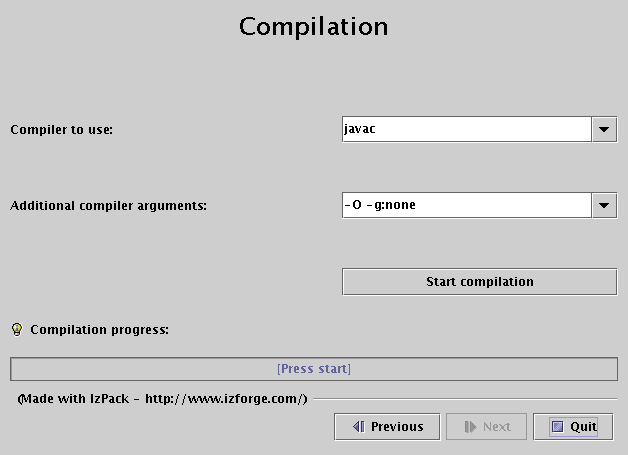
\includegraphics[width=\linewidth]{img/compilePanel}

\subsection{ProcessPanel}

This panel allows you to execute arbitrary files after installation.
The details for the compilation are specified using the resource \texttt{ProcessPanel.Spec.xml}.

The XML file has the following format:
\begin{verbatim}
<processing>
  <job name="do xyz">
    <os family="windows" />
    <executefile name="$INSTALL_PATH/scripts/xyz.bat">
      <arg>doit</arg><arg>$variable</arg>
    </executefile>
  </job>
  <job name="do xyz">
    <os family="unix" />
    <executefile name="$INSTALL_PATH/scripts/xyz.sh">
      <arg>doit</arg><arg>$variable</arg>
    </executefile>
  </job>
</processing>
\end{verbatim}

Each job may have an \texttt{<os>} attribute -- see \ref{tag:os} for details.\\

It is also possible to execute Java classes from this panel. Here's what this
feature author (Alex Bradley) says:
\begin{quotation}
I've been able to work around my requirements by extending the
\texttt{ProcessPanelWorker} functionality to run user-specified classes. I've
extended the DTD of the \texttt{ProcessPanel.Spec.xml} to include a new element:
\begin{verbatim}
<executeclass name="classname">
<args..../>
</executeclass>
\end{verbatim}
I've also added a new sub-class of \texttt{Processable} called
\texttt{executeclass}. This will run a user-specified class in the context of
the installer JVM with a single method :
\begin{verbatim}run( AbstractUIProcessHandler handler, String[] args]);\end{verbatim}

It can do everything I need and more. In particular, it allows me to write a
process extension and still be able to provide feedback to the user through
the feedback panel, and to add new functionality to the installer, after its
been built.
\end{quotation}

New with version 3.7 is the possibility to tee output that is written to
the ProcessPanel's textarea into an optional logfile. Using this feature is
pretty much straightforward, you only have to add a line in \texttt{ProcessPanel.Spec.xml} 
that will tell IzPack the location, where the logfile should be stored.

Variable substitution is performed, so you can use \texttt{\$INSTALL\_PATH} as example.

The name of the logfile is not (yet) configurable but should fit in most cases. It will
be named 
\begin{verbatim}
Install_V<$APP_VER>_<YYYY>-<MM>-<DD>_<hh>-<mm>-<ss>_<RandomId>.log
\end{verbatim}

Here's an example:

\begin{verbatim}
<processing>
  <logfiledir>$INSTALL_PATH</logfiledir>
  <job name="do xyz">
    <os family="windows" />
    <executefile name="$INSTALL_PATH/scripts/xyz.bat">
      <arg>doit</arg><arg>$variable</arg>
    </executefile>
</processing>
\end{verbatim}

This will generate a logfile named e.g. \texttt{Install\_V1.3\_2004-11-08\_19-22-20\_43423.log} 
located in \texttt{\$INSTALL\_PATH}.

\texttt{ProcessPanelWorker} will write all output that is directed to \texttt{stdout} and \texttt{stderr} to this file
if \texttt{ProcessPanel.Spec.xml} contains the \texttt{logfiledir} entry.

Please note that this one file is used for storing the complete output of all jobs and not
a file for each job that is run.

\subsection{JDKPathPanel}
This panel allows the user to select a JDK path. The variable JAVA\_HOME does
not point to a JDK, else to a JRE also the environment variable points to a JDK.
This is not a bug, this is the behavior of the VM. But some products needs a JDK,
for that this panel can be used. There is not only a selection of the path else 
a validation. The validation will be done with the file JDKPath/lib/tools.jar.
If JAVA\_HOME points to the VM which is placed in the JDK, the directory will 
be used as default (JAVA\_HOME/..). If there is the variable
\begin{verbatim}
JDKPathPanel.skipIfValid
\end{verbatim}
defined with the value "yes", the panel will be skiped if the path is valid.
Additional it is possible to make a version control. If one or both variables
\begin{verbatim}
JDKPathPanel.minVersion
JDKPathPanel.maxVersion
\end{verbatim}
are defined, only a JDK will be accepted which has a version in the
range of it. The detection is a little bit pragmatically, therefor it is 
possible, that the detection can fail at some VMs. 
The values in the install.xml should be like 
\begin{verbatim}
<variables>
  <variable name="JDKPathPanel.minVersion" value="1.4.1" />
  <variable name="JDKPathPanel.maxVersion" value="1.4.99" />
  <variable name="JDKPathPanel.skipIfValid" value="yes" />
</variables>
\end{verbatim}

If all is valid, the panels isValidated method sets the variable
\begin{verbatim}
JDKPath
\end{verbatim}
to the chosen path. Be aware, this variable exist not until the JDKPanel
was quitted once. At a secound activation, the default will be the
last selection.
